\begin{ccHtmlOnly}
<center>
<img border=0 src="./saarhull.gif" align=middle>
</center>
\end{ccHtmlOnly} 

\begin{ccTexOnly}
\begin{center}
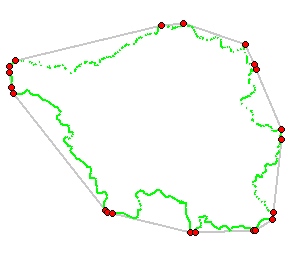
\includegraphics[width=6.5cm]{Convex_hull_2/saarhull}
%\leavevmode\epsfxsize8cm\epsffile{Convex_hull_2/saarhull.eps}
\end{center}
\end{ccTexOnly}

\section{Convex Hull}
\label{sec:convex_hull_2}
\cgal\ provides implementations of several classical algorithms for
computing the counterclockwise sequence of extreme points for a set of 
points in two dimensions (\textit{i.e.}, the counterclockwise sequence 
of points on the convex hull).  The algorithms have different asymptotic
running times and require slightly different sets of geometric primitives. 
Thus you may choose the algorithm that best fits your setting.

Each of the convex hull functions presents the same interface to the
user.  That is, the user provides a pair of iterators, \ccc{first}
and \ccc{beyond}, an output iterator \ccc{result},  and a traits class
\ccc{traits}. The points in the range [\ccc{first}, \ccc{beyond}) define
the input points whose convex hull is to be computed.  The counterclockwise
sequence of extreme points is written to the sequence starting at position
\ccc{result}, and the past-the-end iterator for the resulting set of
points is returned.  The traits classes for the functions specify the types
of the input points and the geometric primitives that are required by
the algorithms. All functions provide an interface in which this
class need not be specified and defaults to types and operations defined
in the kernel in which the input point type is defined.

Given a sequence of $n$ input points with $h$ extreme points,
the function \ccc{convex_hull_2}\ccIndexMainItem[C]{convex_hull_2}
uses either the output-sensitive $O(n h)$ algorithm of Bykat \cite{b-chfsp-78}
(a non-recursive version of the quickhull \cite{bdh-qach-96} algorithm)%
\ccIndexSubitem{convex hull, 2D}{quickhull}
\ccIndexSubitem{convex hull, 2D}{Bykat's algorithm} 
or the algorithm of Akl and Toussaint, which requires $O(n \log n)$ time
in the worst case.  The algorithm chosen depends on the kind of 
iterator used to specify the input points.  These two algorithms are
also available via the functions \ccc{ch_bykat} and \ccc{ch_akl_toussaint},
respectively.  Also available are 
the $O(n \log n)$ Graham-Andrew scan algorithm \cite{a-aeach-79,m-mdscg-84} 
(\ccc{ch_graham_andrew}\ccIndexMainItem[C]{ch_graham_andrew}), 
the $O(n h)$ Jarvis march algorithm \cite{j-ichfs-73}
(\ccc{ch_jarvis}\ccIndexMainItem[C]{ch_jarvis}),
and Eddy's $O(n h)$ algorithm \cite{e-nchap-77}
(\ccc{ch_eddy}\ccIndexMainItem[C]{ch_eddy}), which corresponds to the 
two-dimensional version of the quickhull algorithm.
The linear-time algorithm of Melkman for producing the convex hull of 
simple polygonal chains (or polygons) is available through the function
\ccc{ch_melkman}\ccIndexMainItem[C]{ch_melkman}.%
\ccIndexSubitem{convex hull, 2D}{of polyline or polygon}

\section{Example using Graham-Andrew's Algorithm}

In the following example a convex hull is constructed from point data read 
from standard input using \ccc{Graham_Andrew} algorithm. The resulting convex 
polygon is shown at the standard ouput console. The same results could be 
achieved by substituting the function \ccc{CGAL::ch_graham_andrew} by other 
function like \ccc{CGAL::ch_bykat}.

\ccIncludeExampleCode{Convex_hull_2/ch_example_from_cin_to_cout.cpp}


\section{Extreme Points and Hull Subsequences}
In addition to the functions for producing convex hulls, there are a
number of functions for computing sets and sequences of points related
to the convex hull.  
The functions \ccc{lower_hull_points_2}\ccIndexMainItem[C]{lower_hull_points_2}
and \ccc{upper_hull_points_2}\ccIndexMainItem[C]{upper_hull_points_2}
provide the computation of the counterclockwise 
sequence of extreme points on the lower hull and upper hull,
respectively.  The algorithm used in these functions is
Andrew's variant of Graham's scan algorithm \cite{a-aeach-79,m-mdscg-84},
which has worst-case running time of $O(n \log n)$.

There are also functions available for computing certain subsequences 
of the sequence of extreme points on the convex hull.  The function
\ccc{ch_jarvis_march}\ccIndexMainItem[C]{ch_jarvis_march}
generates the counterclockwise ordered subsequence of
extreme points between a given pair of points and
\ccc{ch_graham_andrew_scan}\ccIndexMainItem[C]{ch_graham_andrew_scan}
computes the sorted sequence of extreme points that are
not left of the line defined by the first and last input points.

Finally, a set of functions 
(\ccc{ch_nswe_point}, \ccc{ch_ns_point}, \ccc{ch_we_point}, \ccc{ch_n_point},
\ccc{ch_s_point}, \ccc{ch_w_point}, \ccc{ch_e_point})
is provided for computing extreme points of a 
2D point set in the coordinate directions.%
\ccIndexSubitem{extreme points, 2D}{in coordinate directions}
